
\subsubsection{22.10.14}

\begin{enumerate}
	\item Время начала и окончания собрания:\newline
	18:00 - 21:40
	\item Цели собрания:\newline
	\begin{enumerate}
	  \item Разобраться, в чем причина поломки направляющей.\newline
	  
	  \item Отремонтировать направляющую.\newline
	  
	  \item Понять, каким образом можно не допустить подобной поломки в дальнейшем.\newline
	  
    \end{enumerate}
    
	\item Проделанная работа:\newline
	\begin{enumerate}
	  \item После тщательного исследования конструкции подъемника было выяснено, что поломка произошла вследствие создания избыточного напряжения из-за стягивания двух направляющих друг с другом поперечным ребром жесткости. Было решено увеличить расстояние между двумя соответствующими направляющими, заменив прослойку между ребром жесткости и направляющими с шайб на более толстые гайки.\newline
      
      \item Починить мебельную рейку не удалось, поэтому она была заменена на точно такую же, оставшуюся после отказа от лишней пары реек при создании подъемника.\newline
      
      \item После того, как ребро жесткости было закреплено на роботе так, что прослойки из гаек были поставлены с обоих сторон, было обнаружено, что теперь направляющие слишком сильно распираются поперечной балкой. Тогда было решено оставить гайки только с одной стороны, в то время как с другой вернуть изначальную прослойку из шайб. После этого было достигнуто состояние, в котором направляющие не испытывают негативного поперечного воздействия.\newline
      
      \begin{figure}[H]
      	\begin{minipage}[h]{1\linewidth}
      		\center{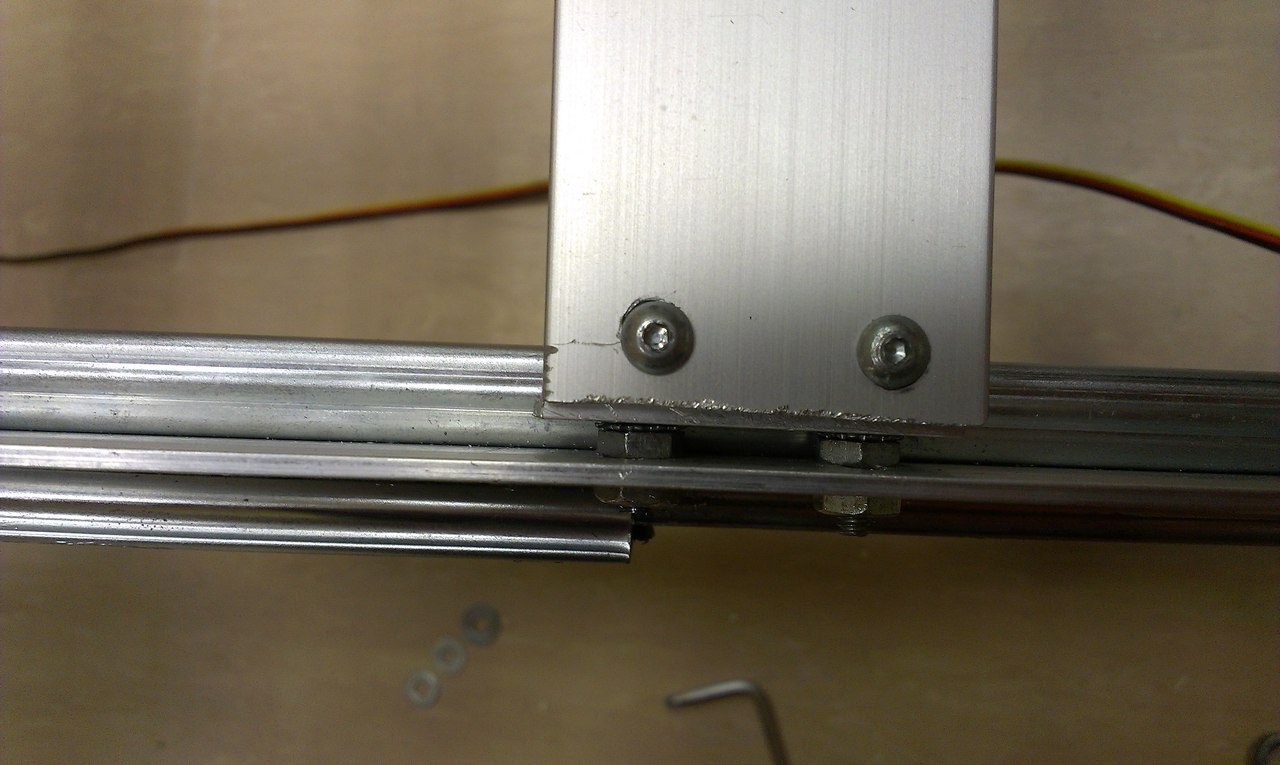
\includegraphics[height=0.9\measurepage]{days/22.10.14/images/01}}
      		\caption{Прослойка между ребром жесткости и направляющей}
      	\end{minipage}
      \end{figure}
      
      \item Не смотря на то, что проблема была устранена, на всякий случай было решено приобрести запасные направляющие, поскольку сломанные рейки уже не поддаются восстановлению.\newline
      
      \item Помимо всего прочего, было создано крепление для перекладины, которая будет располагаться на внутренней паре реек.\newline
      
      \begin{figure}[H]
      	\begin{minipage}[h]{1\linewidth}
      		\center{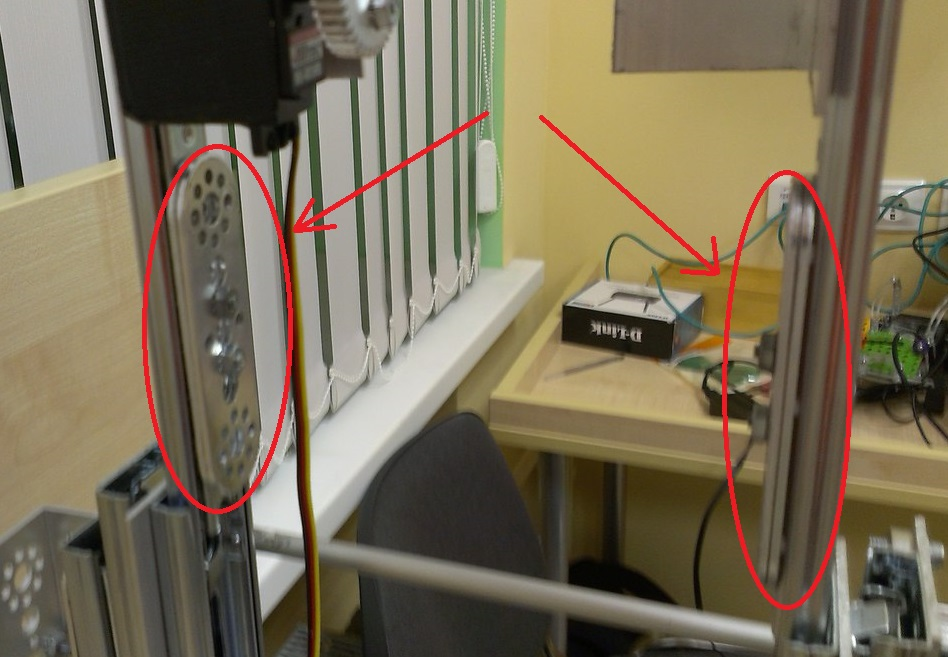
\includegraphics[width=1\linewidth]{days/22.10.14/images/02}}
      		\caption{Крепление для внутренней перекладины}
      	\end{minipage}
      \end{figure}
      
    \end{enumerate}
    
	\item Итоги собрания: \newline
	\begin{enumerate}
	  \item Ремонт подъемника выполнен.\newline
	  
      \item Создано крепление для внутренней рейки.\newline
      
    \end{enumerate}
    
	\item Задачи для последующих собраний:\newline
	\begin{enumerate}
	  \item Приобрести запасные мебельные рейки.\newline
	  
    \end{enumerate}     
\end{enumerate}

\fillpage
